\chapter{Introduction}
\addcontentsline{toc}{chapter}{Introduction} 

%\subsection{Motivation}
%\label{subsec:label}

In this first chapter, we introduce the reader to the research context and background of the thesis. Afterwards, we situate this work within the research line of our group, and finally we describe the proposed objectives. 

\section{Research context}
\label{sec:introduction_research_context}

\subsection{Multiple Sclerosis}
\label{sub:introduction_multiple_sclerosis}

The human nervous system can be divided into the central nervous system (CNS) consisting on the brain and the spinal chord, and the peripheral nervous system, which connects the CNS with the sense organs \cite{Brodal2010}. CNS is mainly constituted by two tissue components: gray matter (GM), which consists of neuronal cell bodies; and white matter tissue (WM), which is mainly composed of myelinated axon tracts \cite{Sperber2006}. In the case of the brain,  it is mostly composed by GM and WM, both evolved by the Cerebro-spinal fluid (CSF), which provides basic mechanical and immunological protection to the brain inside the skull \cite{Sperber2006}. 

Multiple sclerosis (MS) is the most common chronic immune-mediated disabling neurological disease of the CNS \cite{Steinman1996}, in which the insulating covers of the nerve cells in the spinal chord and brain are damaged \cite{Compston2008}. Nowadays, MS is the most frequent non-traumatic neurological disease that causes more disability in young adults. It follows a similar behavior also seen in other putative autoimmune diseases, and affects twice as many women as it does in men \cite{Confavreux1980}. It has a low incidence in childhood, but it increases rapidly in adulthood reaching a peak between 25 and 35 years, and then slowly declines, becoming rare at 50 and older \cite{Cabezas2011}. So far, the world estimate for the disease is between 1.3 to 2.5 million cases, being relatively common in Europe, the United States, Canada, New Zealand, and parts of Australia, but rare in Asia, and in the tropics and subtropics of all continents \cite{Cabezas2011}. 

MS is characterized by areas of inflammation, demyelination, axonal loss, and gliosis scattered throughout the CNS, often causing motor, sensorial, vision, coordination, deambulation, and cognitive impairment \cite{Compston2002}. Demyelination is the process of progressive damage to the protective covering (myelin sheat) around the axon of the neurons. Demyelinated axons conduct impulses at reduced or spontaneous velocity causing impairment in sensation, movement and cognition \cite{Compston2008}. The different clinical courses of the disease are generally grouped in four subtype forms \cite{Lublin1996}. The  \textit{Relapsing/Remitting} (RRMS) form of the disease is characterized by exacerbation times where symptoms are present. These periods are followed by periods of remission, where the patient recovers partial or totally from the disease symptoms. The \textit{Secondary Progressive} (SPMS) form is characterized by a gradual intensification of symptoms between affection relapses. The \textit{Progressive remitting} (PRMS) form is typified by an increase in the relapsing times with significant recovery but with worsening symptoms in new relapsing intervals. Lastly, the \textit{Primary Progressive} (PPMS) form is characterized by a severe decrease of remitting times with special localization in the brain. In general, 50\% of RRMS patients after 10 years develop the SPMS form of the disease. After 25 years, the 90\% of RRMS patients would develop the SPMS form. 


%MRI images are created by computing mathematical inverse transformations of the energy released by hydrogen ions being exposed to different magnetic fields and radio waves. 
\subsection{Magnetic resonance imaging in MS}
\label{subsec:introduction_magnetic_resonance_imaging}
Magnetic Resonance Imaging (MRI) is a noninvasive medical imaging technique that is used in radiology to generate image representations of different internal anatomical organs and physiological processes of the body. Over the last 40 years, MRI have evolved as a clinical modality \cite{Geva2006}, and in particular as an essential tool for the diagnosis and evaluation of central nervous system disorders such as MS \cite{Edelman1993}. On MRI, MS plaques are well-delimited regions with hypo-intense signal intensity with respect to GM on T1-weighted (T1-w), while hyper-intense with respect to GM on T2-weighted (T2), Proton Density (PD) and Fluid Attenuated Inversion Recovery (FLAIR) modalities (see Figure \ref{mri_modalities}).

\begin{figure*}[top]
  \begin{center}
    %\vspace{-3cm}
    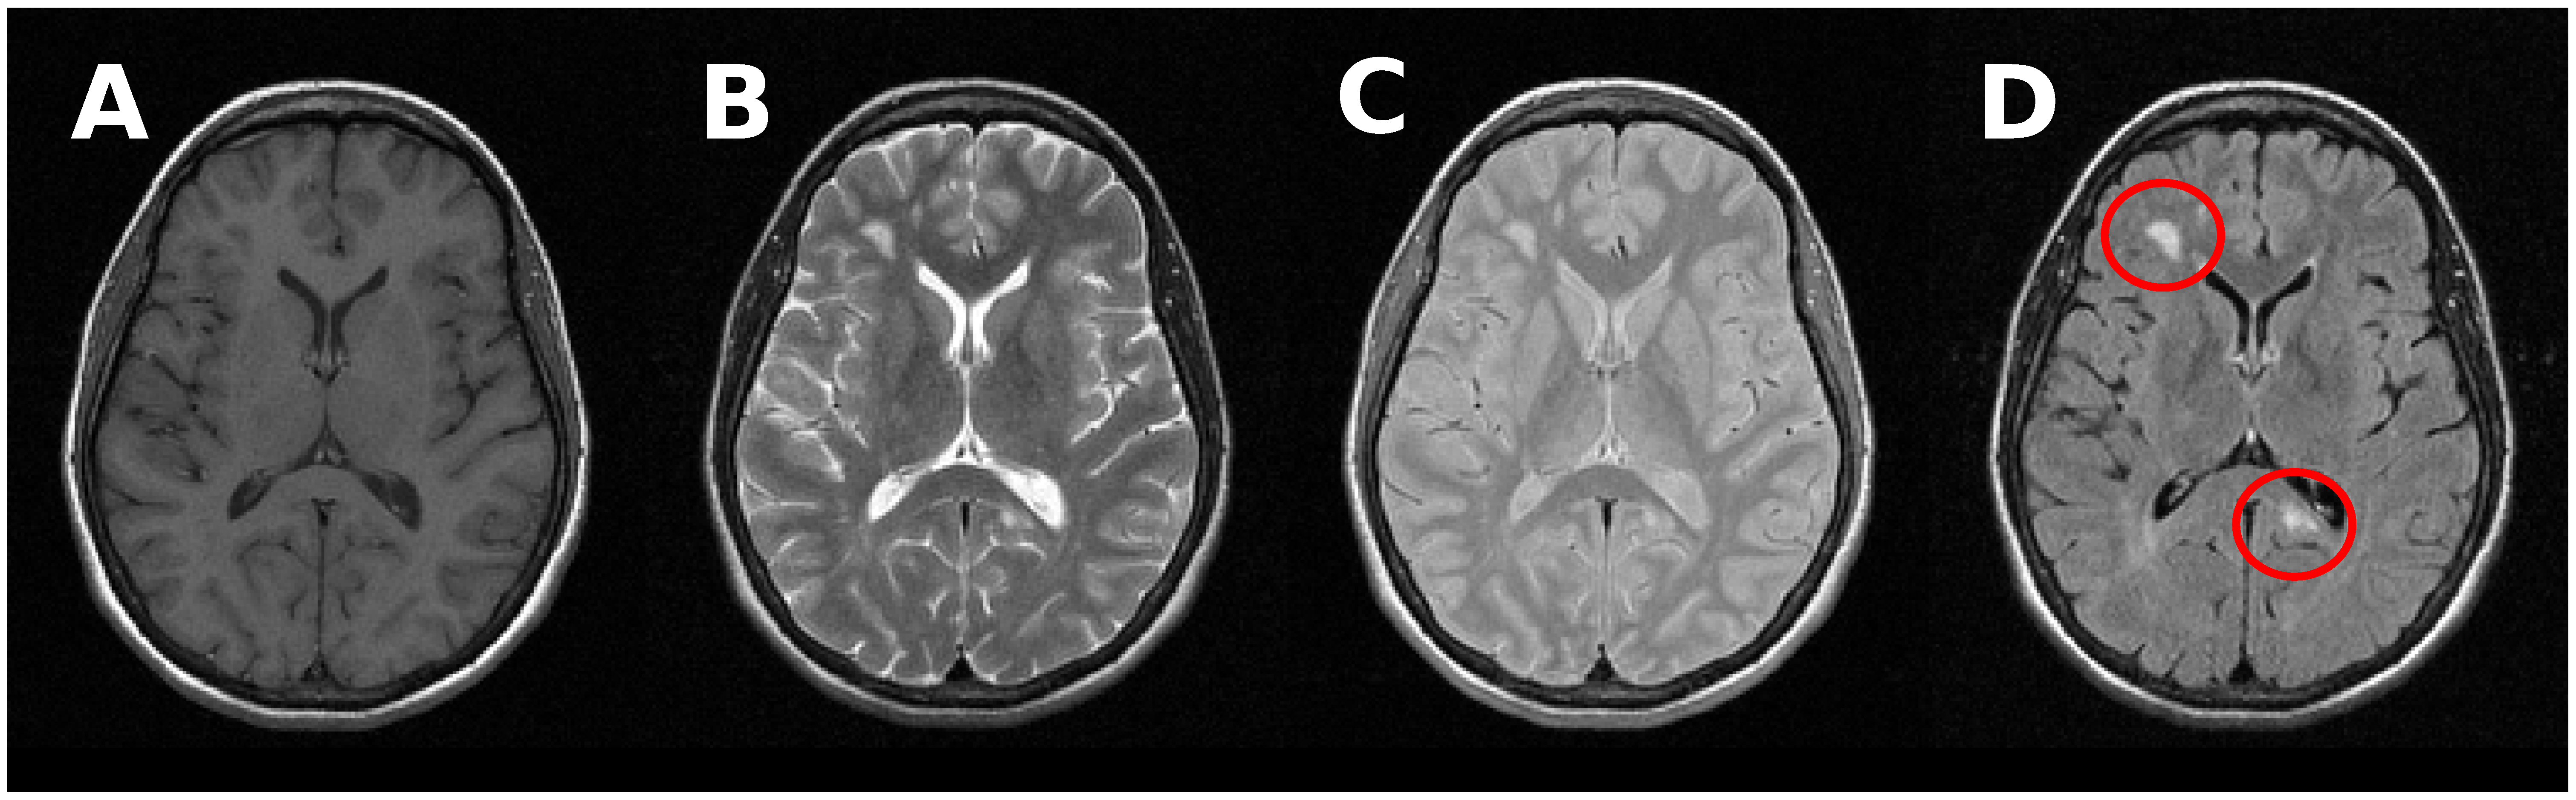
\includegraphics[width=1\textwidth]{figures/figure_1.eps}
  \end{center}
    \caption{MRI image modalities. A) T1-weighted (T1-w) image sequence. B) T2-weighted (T2-w) image sequence. C) Proton Density (PD) image sequence. D) Fluid Attenuated Inversion Recovery (FLAIR) sequence. MS plaques are shown inside red circles on the FLAIR modality. MS plaques are hypo-intense with respect to GM and WM in T2-w, PD and FLAIR sequences, while hypo-intense with respect to WM on the T1-w modality.}
    \label{mri_modalities}
\end{figure*}

In this aspect, new criteria for MS diagnosis and monitoring has been revised in the last years \cite{Polman2011}, due to the MRI sensitivity to reveal focal white matter (WM) lesion plaques and disease activity in time and space \cite{Filippi2011}. Additionally, various studies have also analyzed the correlation between MRI brain tissue atrophy measures and MS disability status, showing that tissue loss is an important component of the disease progression \cite{Chard2002, Filippi2013, Fisher2008, Rudick2009}. Tissue loss seems to increase through the course of MS with a similar rate between 0.3\% and 0.5\% per year, and independently of the MS subtype \cite{DeStefano2010, Rudick2009}. In general, GM atrophy is more associated with disability changes than WM atrophy \cite{Fisniku2008}, and not only in the RRMS and SPMS MS subtypes \cite{Fisher2008, Rudick2009}, but also in CIS patients where several studies have shown a significantly greater ventricular cavities and an associated GM loss on MRI scans of CIS patients that will develop MS compared to those who not \cite{Ceccarelli2010,Filippi2013}.

\subsection{Image analysis in MS}
\label{subsec:image_analysis}

Manual analysis of brain images is unfeasible in practice, given the large number of three-dimensional MRI slices for each patient and the possible intra/inter observer variability between experts \cite{Cabezas2011}. This has led to the development since the early nineties of a wide number of lesion and tissue segmentation methods, with the aim to reduce the execution time and the inherent variability of manual annotations \cite{Cline1990, Gerig1992, Kapur1996}. 


\subsubsection{Pre-processing of MRI images}
Acquired brain MRI volumes incorporate non brain tissue parts of the head such as eyes, fat, spinal cord or brain skull. Brain tissue extraction from non-brain tissue is commonly referred in the literature as skull-stripping (see Figure \ref{preprocessing_mri} B and C). Skull-stripping has a direct effect on the performance of automated methods, as differences in skull stripping would lead into unexpected results in the tissue classification if skull or eyes are included as brain tissue \cite{Acosta-Cabronero2008, Popescu2012}. Among the different proposed methods for skull-stripping \cite{Acosta-Cabronero2008, Lee2003, Roura2014}, the Brain Extraction Tool (BET) \cite{Smith2002}, and the Brain Surface Extractor (BSE) \cite{Shattuck2001} are the most commonly used methods by the neuro-imaging community.

Furthermore, inherent characteristics of the MRI acquisition process such as differences in the magnetic field, bandwidth filtering of the data or eddy currents driven by field gradients usually derive in image artifacts that may also have a negative impact on the performance of methods \cite{Simmons1994}. In these cases, intensity correction of MRI images is either performed before lesion/tissue segmentation, or as an integrated part of the tissue segmentation pipeline  (see Figure \ref{preprocessing_mri} D). Among the former available strategies proposed \cite{Arnold2001,Hou2006}, the N3 \cite{Sled1998}, and N4 \cite{Tustison2010} methods are currently the de-facto standard tools used for intensity correction. 


\begin{figure*}[top]
  \begin{center}
    %\vspace{-3cm}
    \includegraphics[width=1.0\textwidth]{figures/figure_2.eps}
  \end{center}
    \caption{MRI pre-processing steps. A) T1-weighted (T1-w) image sequence. B) Computed brain mask and C) skull stripped T1-w sequence using the BET approach \cite{Smith2002}. D) Estimated T1-w bias-field using the N3 method proposed by \cite{Sled1998}.}
    \label{preprocessing_mri}
\end{figure*}

\subsubsection{Automated lesion segmentation}

MRI based diagnostic criteria for MS has led to an increasing need to analyze quantitatively focal MS lesions in individual and temporal studies \cite{Cabezas2014, Polman2011}. Different sequences such as T2-w, PD and FLAIR are often used in lesion classification, as MS lesions appear brighter than GM and WM on them. However, WM lesions often present a similar signal intensity profile to CSF on T2-w. In contrast, FLAIR sequences suppress fluids from the image, restraining the CSF tissue effects on the acquired image, although some severe T2-w hyper-intense lesions appear similar to CSF in FLAIR \cite{Harmouche2015}. 

A wide number of automated lesion segmentation techniques have been proposed during the last years \cite{Garcia-Lorenzo2013, Llado2012}. In these methods, classification is based either in supervised or unsupervised learning. Supervised learning methods employ a training set of correctly-identified observations that are used as prior information to learn the lesion characteristics. Newer proposed strategies integrate spatial decision forest \cite{Geremia2011}, statistical methods \cite{Sweeney2013}, patch-based models \cite{Guizard2015} or adaptive dictionary learning strategies \cite{Deshpande2015}. In contrast, unsupervised learning methods do not use any prior information in the classification task, which involves grouping data into categories based on some measure of inherent similarity or distance characteristic of the input images. Among these, most recent methods include probabilistic models which separate WM lesions from normal-appearing tissue by considering lesions as an outlier class \cite{Harmouche2015,Jain2015,Tomas-Fernandez2015}, or techniques that make use of the signal intensity of lesions on FLAIR to apply several thresholding methods with post-processing steps to automatically segment lesions \cite{Roura2015, Schmidt2012}. 


\subsubsection{Automated brain tissue segmentation in MS}
\label{subsec:lesion_segmentation}
The existent correlation between brain tissue atrophy measures and MS disability status \cite{Filippi2013, Fisher2008}, has increased the necessity to develop robust automated brain tissue segmentation methods capable to perform accurate brain tissue volume measurements \cite{Giorgio2013}. However, automated segmentation of brain tissue is still a challenging problem due to the complexity of the images, existence of lesions, differences in tissue intensities, noise, intensity inhomogeneities and the absence of models of the anatomy that fully capture the possible deformations in each structure \cite{Cabezas2011, Kapur1996}. 

A wide number of brain tissue segmentation methods have been proposed so far. General purpose intensity based methods usually perform tissue segmentation on T1-w sequences, as this modality clearly separates gray matter from white matter. These include probabilistic strategies based on Bayesian inference \cite{Ashburner2005,Marroquin2002, Roy2012,Shattuck2001}, Markov Random Fields models \cite{Bricq2008, Tohka2010, Zhang2001}, or unsupervised clustering methods such as Zhang2001, \textit{Fuzzy logic} \cite{Caldairou2011, Pham2001}. In contrast, supervised learning approaches also combines T1-w sequences with other modalities such as T2-w and PD using \textit{K-Nearest-Neighbor} classifiers \cite{deBoer2009,Vrooman2013}, \textit{Support Vector Machines} \cite{Akselrod2006,Opbroek2013}, \textit{Random Forests} \cite{yi2009,Mahapatra2014}, or trained \textit{Gaussian mixture models} \cite{Rajchl2015}. 

However, different studies \footnote{Em puc referenciar jo AJNR2015?} have shown that tissue abnormalities found in MS image patients such as WM lesions reduce the accuracy of tissue segmentation methods \cite{Battaglini2012, Chard2010}. Effectively, WM lesions on T1-w are hypo-intense with respect to normal-appearing WM, and  therefore, lesion voxels that are classified as GM are distorting the overall GM volume. However, lesion voxels may also have an effect in the observed differences in normal-appearing tissue. WM lesions which are actually classified as WM decrease the mean overall signal intensity of the WM, causing that GM voxels with signal intensities similar to WM lesions may be also mis-classified as WM.  In contrast, if WM lesions are classified as GM, normal-appearing WM voxels with signal intensities similar to lesions may be miss-classified as GM. 
 
\subsubsection{Lesion filling}
\label{subsec:lesion_filling}
In MS, hypo-intense WM lesions have to be pre-processed before tissue segmentation in order to reduce the effects of WM lesions on tissue segmentation. Historically, WM lesions have been masked-out of the T1-w before segmentation, and their volume have been added to WM afterwards \cite{Chard2002}. Although this method effectively reduces the error in tissue volume, it has been show that this approach is not optimal \cite{Battaglini2012, Chard2010}. 

In this aspect, several strategies have proposed to in-paint lesions on the T1-w with signal intensities of the normal-appearing WM before tissue segmentation \cite{Battaglini2012, Chard2010, Magon2014, Sdika2009}, a process which is usually known in the literature as lesion filling. However, most of the available lesion filling methods require manual delineations of lesions, which may be tedious, challenging and time-consuming task depending of the characteristics of the image \cite{Llado2012}. When available, lesion filling has demonstrated not only a significant reduction in the associated errors of WM lesions in tissue volume measurements \cite{Popescu2014}, but also in image registration \cite{Ceccarelli2012,  Diez2014, Sdika2009} and cortical thickness measurements \cite{Magon2014}. 

\section{Research background}
\label{sec:research_background}

This thesis is located within the framework of different research projects associated to the Computer Vision and Robotics research group (VICOROB), a research institute of the University of Girona\footnote{www.vicorob.udg.edu}. VICOROB has been working on several medical image analysis projects since 1996, mainly in segmentation and registration of mammography images. Lately in 2010, the research group started a fruitful collaboration with several medical MS research teams with the aim to develop new automated techniques capable to segment MS lesions and to perform atrophy measurements that can be transferred to experts for clinical use. In particular, our research in the MS field has been carried out within the following research projects:

\begin{enumerate}

\item $[2009-2012]$ PI09/91918 ``SALEM: Segmentaci\'{o}n Autom\'{a}tica de Lesiones de Esclerosis M\'{u}ltiple en im\'{a}genes de resonancia magn\'{e}tica" awarded by the Instituto Carlos III. 

\item $[2010-2012]$ VALTEC09-1-0025 ``Salem: toolkit para la segmentaci\'{o}n autom\'{a}tica de lesiones de Esclerosis M\'{u}ltiple en resonancia magn\'{e}tica" awarded in 2009 by the Generalitat de Catalunya within the "Projectes de valoritzaci\'{o} VALTEC".

\item $[2015-2017]$ TIN2014-55710-R: ``Herramientas de neuroimagen para mejorar el diagnosis y el seguimiento cl\'{i}nico de los pacientes con Esclerosis M\'{u}ltiple" awarded in 2014 by the spanish call Retos de investigaci\'{o}n 2014.

\item $[2015-2019]$ BiomarkEM.cat: To develop, validate and transfer to clinical practice robust tools and totally automated for measuring new lesions and changes on the brain volume within MS patients. Awarded in 2015 by the Fundaci\'{o} Marat\'{o} de TV3.

\end{enumerate}

Since then, the research group has published original contributions in different fields such as image pre-processing \cite{Roura2014}, MS lesion segmentation \cite{Cabezas2014, Cabezas2014b, Llado2012, Roura2015}, temporal analysis \cite{Ganiler2014,Llado2012b}, image registration \cite{Diez2014, Roura2015b}, and tissue segmentation \cite{Cabezas2011}. All this works have been published in partnership with different medical MS teams from:

\begin{itemize}

	\item from the Hospital Vall d'Hebron: Dr. Rovira, who is the director of the ``Unitat de Resson\`{a}ncia Magn\`{e}tica-Centre Vall d'Hebron" (URMVH) and has participated in several research projects funded by public and private institutions in the last few years, as well as Dr. Pareto and technicians Huerga and Corral. This group is part of the MAGNIMS network, a European network of centres that share an interest in the MS study through MRI.
 
	 \item from the Cl\'{i}nica Girona / Hospital Santa Caterina: Dr. Vilanova and Dr. Barcel\'{o} are the codirectors of the ``Unitat de Resson\`{a}ncia Magn\`{e}tica" at the Cl\'{i}nica Girona and are members of several national and international radiology societies.
 
	\item from the Hospital Josep Trueta: Dr. Rami\'{o}-Torrent\`{a}, who is the current coordinator of the "Unitat de Neuroimmunologia i Esclerosi M\'{u}ltiple", as well as Drs. Robles and Beltr\'{a}n, who work for the radiology unit.

\end{itemize}


\section{Objectives}
\label{sec:objectives}

As part of the TIN2014-55710-R and BiomarkEM.cat research project frameworks, the main goal of this thesis is: 

\begin{center}
	%\fbox{\parbox[c]{0.85\textwidth}{\textbf{the improvement of the current pipeline capable to detect and segment MS lesions in MRI and its integration in a standard platform.}}}
	\fbox{\parbox[c]{0.88\textwidth}{\textbf{to develop a novel fully automated brain tissue segmentation method capable of computing accurate tissue volume measurements of MS patient images.}}}
\end{center}

\noindent This objective refers to the brain tissue segmentation of MS patient images at a specific time but we do not consider the differences in tissue volume at different stages. 

Different stages have to be covered first in order to fulfill the main proposed goal. The aim of each of the proposed stages is to permit us to gain a better knowledge of the different parts that compose a fully automated tissue segmentation method for MS images containing lesions. Hence, we detail each of the proposed stages to cover: 

\begin{itemize}

\item \textbf{to analyze the state of the art of tissue segmentation methods}. The first stage aims to review different proposed tissue segmentation techniques in order to understand their advantages and drawbacks. Methods are evaluated on public databases that incorporate manual tissue annotations, which permits to perform a quantitative analysis of the accuracy of the methods.
  
\item \textbf{to study the effect of WM lesions on tissue segmentation of MS patient images}. Although it is know that the inclusion of WM lesions on tissue segmentation distort the brain volume measurements, this effect has not been studied and compared across different tissue segmentation methods. In this aspect, the second stage is focused on the analysis of the effects of WM lesions on the tissue distributions of a set of tissue segmentation approaches using multi-center 1.5T MS data from different scanners. Our hypothesis here is that a better knowledge of the correlation between lesion attributes, such as signal intensity and lesion size, and the observed differences in tissue volume of the analyzed algorithms may be beneficial to design a tissue segmentation method for MS. 

\item \textbf{to reduce the effect of WM lesions on tissue segmentation of MS patient images}. As said in section \ref{subsec:lesion_filling}, WM lesions have to be pre-processed before tissue segmentation in order to reduce the effects of WM lesions on tissue segmentation. In this aspect, the third stage is two-fold: first, to compare the accuracy of different proposed lesion filling techniques in the literature, analyzing their accuracy on both 1.5T and 3T data. Once we have analyzed the benefits and drawbacks of each proposed method, we aim to propose a new lesion filling pipeline in order to overcome the possible limitations of existent methods. The proposed method will be available for the research community. 

\item \textbf{to analyze the effect of automated WM lesion segmentation and filling on the tissue segmentation}. Although lesion filling techniques have already been successfully applied to reduce the effect of WM lesions on tissue segmentation, usually WM lesions are annotated manually before segmentation. In contrast, the effect of both automated lesion segmentation and filling on tissue segmentation is still unclear. The fourth stage of the thesis aims to understand the effects of the inherent errors in automated lesion segmentation on the posterior lesion filling and tissue segmentation. Thus, we aim to compare the accuracy of different state-of-the-art fully automated pipelines that incorporate lesion segmentation, lesion filling and tissue segmentation on MS data, in order to analyze the extend of the effect of remaining lesions on the differences in tissue segmentation, which may be beneficial to update our acquired knowledge in previous stages. 

\item \textbf{to propose a new fully automated tissue segmentation method for MS patient images}. Finally, we aim to benefit from the acquired knowledge on previous stages to propose a \textbf{fully automated tissue segmentation method} able to deal with images of MS patients with different level of brain atrophy and lesion load. In this last stage, we aim to validate the accuracy of the proposed method by comparing it with the state of the art in tissue segmentation in MS. The proposed method will be publicly available for the research community. 

 \end{itemize}


\subsection{Document structure}
\label{sec:label}

A graphical description of the structure of the thesis is shown in Figure \ref{document_structure}. Connections between chapters in Figure \ref{document_structure} depict the conceptual link between chapters :(. The rest of the document is organized as follows:

\begin{figure*}[top]
  \begin{center}
%    \vspace{-3cm}
    \includegraphics[width=1\textwidth]{figures/document_schema.eps}
  \end{center}
    \caption{Organization of the document. Preliminary chapter 1 describes the research context and the main objectives of this thesis. Chapters 2 to 6 introduce the main contributions of this work. Chapter 7 proposes a general discussion of the results obtained in Chapters 2 to 6. Finally, the main conclusions and the proposed future work are defined in Chapter 8. Connections between chapters depict a conceptual link between chapters.}
    \label{document_structure}
\end{figure*}


\begin{itemize}
%\item \textbf{Chapter 1. Introduction.} This chapter has described the research context and the main objectives of this thesis.
\item \textbf{Chapter 2. Comparison of 10 brain tissue segmentation methods using revisited IBSR annotations.}  In chapter 2, we present a comprehensive comparison of the accuracy of 10 brain tissue segmentation methods on two public MRI databases. 
\item \textbf{Chapter 3. Evaluating the Effects of White Matter Multiple Sclerosis Lesions on the Volume Estimation of 6 Brain Tissue Segmentation Methods.} After reviewing different tissue segmentation techniques in public data, we perform a detailed analysis of the effects of WM lesions on the brain tissue volume measurements of six of these tissue segmentation methods using MS data from different hospital centers. 
\item \textbf{Chapter 4. A white matter lesion-filling approach to improve brain tissue volume measurements.} In this chapter, we propose a new technique to fill WM lesions on 1.5T and 3T data, validating its accuracy with other proposed methods in the literature. 
\item \textbf{Chapter 5. Quantifying brain tissue volume in multiple sclerosis with automated lesion segmentation and filling.} In this chapter we present a detailed evaluation of the performance of different automated pipelines that incorporate lesion segmentation, lesion filling and tissue segmentation on MS data. 
\item \textbf{Chapter 6. Automated brain tissue segmentation of MR images in the presence of white matter lesions.} We propose a novel fully automated tissue segmentation pipeline designed to deal with MS patient images containing lesions. We validate the accuracy of the proposed method with other state-of-the-art techniques.   

\item \textbf{Chapter 7. Results and discussion.} This chapter provides an comprehensive discussion of the results obtained in the different performed analyses and proposed methods suggested in this thesis.
\item \textbf{Chapter 8. Conclusions and future work.} Finally, the main conclusions based on the contributions of this thesis are defined. Based on this conclusions, we  summarize different future works to improve or extend the suggested approach.   
\end{itemize}

%%% Local Variables:
%%% mode: latex
%%% TeX-master: "../main"
%%% End:
